\section*{Solutions~4.1}%\ref{S-sets-1}}

\begin{solutions}
	% 1
	\solution
		The possibilities are 2,3,4 and 5 different elements.
		\begin{itemize}
			\item 2: In the case that $a=b=c$. Then the set can be written as: \[\{a, a, \{a\}, \{a, a\}, \{a,a,a\}\}=\{a, \{a\}\}\]
			\item 3: In the case that $a=b\neq c$. Then the set can be written as: \[\{a, a, \{a\}, \{a, c\}, \{a,c\}\}=\{a, \{a\}, \{a, c\}\}\]
			\item 4: In the case that $a\neq b$ and $a=c$. Then the set can be written as: \[\{a, b, \{a\}, \{a, a\}, \{a,b,a\}\}=\{a, b, \{a\}, \{a, b\}\}\]
			\item 5: In the case that $a\neq b\neq c$. Then the set can be written as: \[\{a, b, \{a\}, \{a, c\}, \{a,b,c\}\}\].
		\end{itemize}

	% 2
	\solution
		\spart $A \cup B = \{a,b,c\}; A \cap B = \emptyset; A \SETDIFF B = \{a,b,c\}$
		\spart $A \cup B = \{1,2,3,4,5,6,8,10\}; A \cap B = \{2,4\}; A \SETDIFF B = \{1,3,5\}$
		\spart $A \cup B = \{a,b,c,d\}; A \cap B = \{a,b\}; A \SETDIFF B = \emptyset$
		\spart $A \cup B = \{a,b,\{a\},\{a,b\}\}; A \cap B = \{\{a,b\}\}; A \SETDIFF B = \{a,b\}$

	% 3
	\solution
		\spart 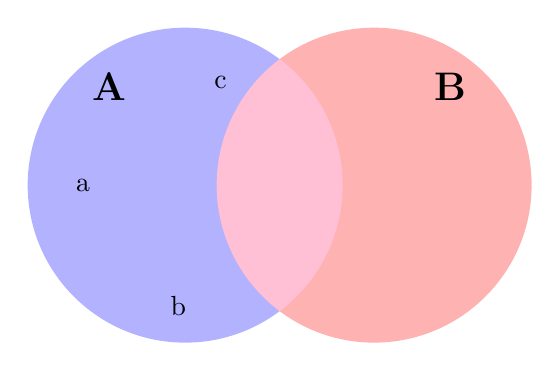
\begin{tikzpicture}
			\begin{scope}[blend group=soft light]
				\fill[red!30!white] (0:1.2) circle (2);
				\fill[blue!30!white]  (180:1.2) circle (2);
			\end{scope}
			
			\node at (150:2.5)	{\Large\textbf{A}};
			\node at (30:2.5)	{\Large\textbf{B}};
			\node at (180:2.5)  {a};
			\node at (230:2)    {b};
			\node at (120:1.5)  {c};
		\end{tikzpicture}
		\spart 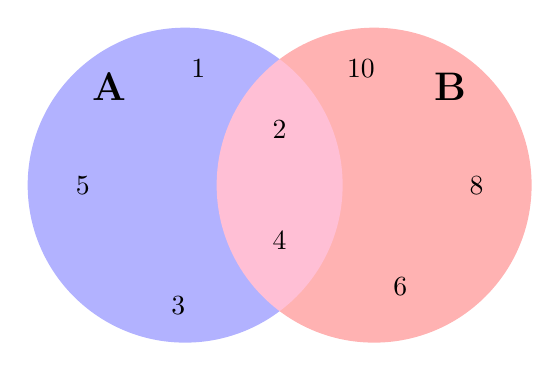
\begin{tikzpicture}
		\begin{scope}[blend group=soft light]
		\fill[red!30!white] (0:1.2) circle (2);
		\fill[blue!30!white]  (180:1.2) circle (2);
		\end{scope}
		
		\node at (150:2.5)	{\Large\textbf{A}};
		\node at (30:2.5)	{\Large\textbf{B}};
		\node at (180:2.5)  {5};
		\node at (230:2)    {3};
		\node at (125:1.8)  {1};
		\node at (90:0.7)   {2};
		\node at (270:0.7)  {4};
		\node at (55:1.8)   {10};
		\node at (0:2.5)    {8};
		\node at (320:2)    {6};
		\end{tikzpicture}
		\spart 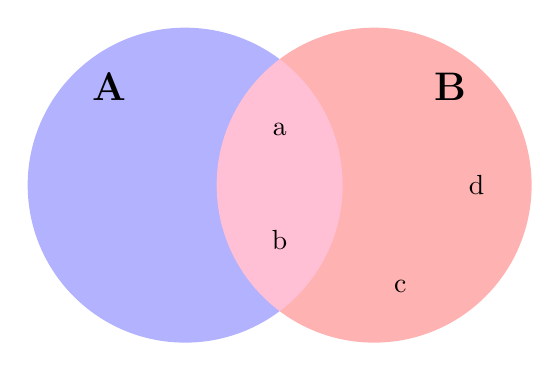
\begin{tikzpicture}
		\begin{scope}[blend group=soft light]
		\fill[red!30!white] (0:1.2) circle (2);
		\fill[blue!30!white]  (180:1.2) circle (2);
		\end{scope}
		
		\node at (150:2.5)	{\Large\textbf{A}};
		\node at (30:2.5)	{\Large\textbf{B}};
		\node at (90:0.7)   {a};
		\node at (270:0.7)  {b};
		\node at (0:2.5)    {d};
		\node at (320:2)    {c};
		\end{tikzpicture}
		\spart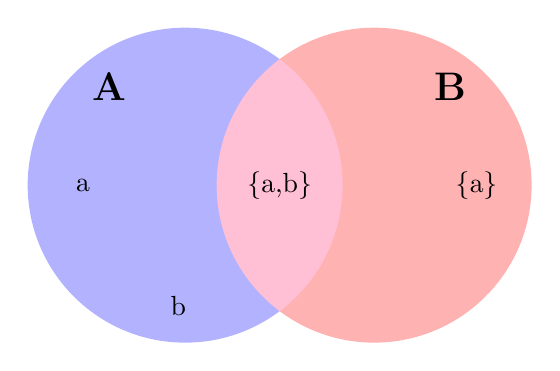
\begin{tikzpicture}
		\begin{scope}[blend group=soft light]
		\fill[red!30!white] (0:1.2) circle (2);
		\fill[blue!30!white]  (180:1.2) circle (2);
		\end{scope}
		
		\node at (150:2.5)	{\Large\textbf{A}};
		\node at (30:2.5)	{\Large\textbf{B}};
		\node at (180:2.5)  {a};
		\node at (230:2)    {b};
		\node at (90:0)     {\{a,b\}};
		\node at (0:2.5)    {\{a\}};
		\end{tikzpicture}

	% 4
	\solution
		\spart $X\cap Y=\{5,6,7,8,9,10\}$
		\spart $X\cup Y=\mathbb{N}$
		\spart $X\SETDIFF Y=\{11,12,13,...\}$
		\spart $\mathbb{N}\SETDIFF Z=\{1,3,5,...\}$
		\spart $X\cap Z=\{6,8,10,...\}$
		\spart $Y\cap Z=\{0,2,4,6,8,10\}$
		\spart $Y\cup Z=\{0,1,2,3,4,5,6,7,8,9,10,12,14,16...\}$
		\spart $Z\SETDIFF \mathbb{N}=\emptyset$

	% 5
	\solution $\POW(\{1,2,3\})=\{\emptyset, \{1\}, \{2\}, \{3\}, \{1,2\}, \{1,3\}, \{2,3\}, \{1,2,3\}\}$

	% 6
	\solution
		\spart False. Although $b$ is part of the two sets that are elements of $A$, namely $\{b\}$ and $\{a,b\}$, the element $b$ itself is not a part of $A$.
		\spart False. In order for $\{a,b\}$ to be a subset of $A$, both $a$ and $b$ should be elements of $A$. Like we specified in \textbf{a)}, $b\notin A$, hence $\{a,b\}\NOT\SUB A$.
		\spart True. In order for $\{a,b\}$ to be a subset of $B$, both $a$ and $b$ should be elements of $B$, which they are.
		\spart False. Although $a$ and $b$ are both individual elements of $B$, the combined set $\{a,b\}$ is not.
		\spart False. Although $a$ and $\{b\}$ are both individual elements of $A$, the combined set $\{a,\{b\}\}$ is not.
		\spart True. $\{a, \{b\}\}$ is an element of $B$.

	% 7
	\solution Yes, this is possible.
	\[\POW(\POW(\emptyset))=\POW(\{\emptyset\})=\{\emptyset, \{\emptyset\}\}\]
	\begin{align*}
	\POW(\POW(\{a,b\}))=&\POW(\{\emptyset, \{a\}, \{b\}, \{a,b\}\})\\
	=&\{\emptyset,\\
	&\{\emptyset\},\{\{a\}\}, \{\{b\}\},\{\{a,b\}\},\\
	&\{\emptyset, \{a\}\}, \{\emptyset, \{b\}\}, \{\emptyset, \{a,b\}\}, \{\{a\}, \{b\}\}, \{\{a\}, \{a,b\}\}, \{\{b\}, \{a,b\}\},\\
	& \{\emptyset, \{a\}, \{b\}\}, \{\emptyset, \{a\}, \{a,b\}\},
	\{\emptyset, \{b\}, \{a,b\}\}, \{\{a\}, \{b\}, \{a,b\}\},\\
	&\{\emptyset, \{a\}, \{b\}, \{a,b\}\}\}
	\end{align*}

	% 8
	\solution The sentence "“She likes dogs that are small, cuddly, and cute" talks about dogs that are both small, and cuddly, and cute. Hence, the dogs she likes has to be in the set of small dogs, the set of cuddly dogs and the set of cute dogs. Therefore, the set of dogs she likes is the intersection of the three sets.\\
	On the other hand, the sentence "She likes dogs that are
	small, dogs that are cuddly, and dogs that are cute" talks about dogs that are either small, cuddly, or cute. Hence, the set of liked dogs is the union of these three sets.

	% 9
	\solution $A \cup A = A$ (remember that sets have no duplicates)\\
	$A \cap A = A$ (after all everything in $A$ that is also in $A$, is everything)\\
	$A \SETDIFF A = \emptyset$ (removing from $A$ everything that is in $A$ leaves us nothing)

	% 10
	\solution
	We know that $A\SUB B$. This means that each element of $A$ is in $B$ as well. Therefore, if we take $A\cup B$ we have a set which is equal to $B$, as all elements of $A$ are in $B$. With the same reasoning, $A\cap B$ is equal to $A$, as all elements of $A$ are in $B$. Moreover, because of this, $A\SETDIFF B$ renders the empty set, as no elements are left when removing all elements from $A$ which are in $B$ as well.

	% 11
	\solution
	\begin{proof}
		In order to prove that $C\SUB A\cap B\IFF (C\SUB A\land C\SUB B)$, we have to show that $C\SUB A\cap B\IMP (C\SUB A\land C\SUB B)$ and $(C\SUB A\land C\SUB B)\IMP C\SUB A\cap B$.
		\begin{itemize}
			\item $C\SUB A\cap B\IMP (C\SUB A\land C\SUB B)$:\\
				We assume that $C\SUB A\cap B$. Take an arbitrary element $x$ in $C$. Because $C\SUB A\cap B$, $x$ is in the intersection of $A$ and $B$. Because this is the case, $x$ is in both $A$ and in $B$. Because this holds for an arbitrary element in $C$, it holds for all elements in $C$. Therefore, all elements of $C$ are an element of both $A$ and $B$, and hence $C\SUB A\land C\SUB B$.
			\item $(C\SUB A\land C\SUB B)\IMP C\SUB A\cap B$:\\
				We assume that $C\SUB A$ and $C\SUB B$.Take an arbitrary element $x$ in $C$. Because $C\SUB A$ and $C\SUB B$, $x$ is both in $A$ and in $B$. Because of this, $x$ is in the intersection of $A$ and $B$ ($A\cap B$) as well. Because this holds for an arbitrary element in $C$, it holds for all elements in $C$. Therefore, all elements of $C$ are in $A\cap B$ and hence $C\SUB A\cap B$.
		\end{itemize}
	\end{proof}

	% 12
	\solution
	\begin{proof}
		Assume that $A\SUB B$ and $B\SUB C$, i.e. that $\forall x(x\in A\IMP x\in B)$ and $\forall x(x\in B\IMP x\in C)$. Take an arbitrary element $x$ in $A$. Because $A\SUB B$, $x$ is in $B$ as well. Moreover, because $B\SUB C$, we have that $x$ is in $C$ as well. Because $x$ is an arbitrary element of $A$, it holds for all elements of $A$ that they are in $C$ as well. Therefore, $A\SUB C$.
	\end{proof}

	% 13
	\solution
	\begin{proof}
		Let us assume that $A\SUB B$. Let us take an arbitrary element $a$ in $\POW(A)$. Since $a$ is in the power set of $A$, it is a subset of $A$. From $a\SUB A$, $A\SUB B$ and the previous question, we know that $a\SUB B$. Because of this, $a\in\POW(B)$. Because $a$ is an arbitrary element from $\POW(A)$, this is true for all elements in $\POW(A)$ and hence, $\POW(A)\SUB\POW(B)$.
	\end{proof}

	% 14
	\solution
	\begin{proof}
		We proof this by proof by contradiction. Therefore, assume that $P(M)$ and $P(k)\IMP P(k+1)$. We assume that $P(n)$ is not true for all $n\geq M$. Then there exists at least one number $s\geq n$ for which $P(s)$ is false. Let us take the smallest number $s^*\geq n$ such that $P(s^*)$ is false. Now, because $s^*$ is the smallest number, we have that $s^*-1$ is true. However we know that $P(k)\IMP P(k+1)$ holds for all $k\geq M$, thus also for $s^*-1$. Thus $P(s^*-1)\IMP P(s^*)$ holds, we now have that $P(s^*)$ is true, leading to a contradiction. Therefore, $P(n)$ must be true for all $n\geq M$.
	\end{proof}

	% 15
	\solution
	\begin{proof}
		Let $C(\phi)$ denote the number of connectives in $\phi$, and $V(\phi)$ denote the number of propositional variables. Let $P(\phi)$ be the statement that $V(\phi)\leq C(\phi)+1$, i.e. the number of propositional variables is at most one more than the number of connectives.\\
		\textbf{Base Case:} $V(x)=1$\\
		By the Atoms rule by the definition of $PROP$, $C(\phi)=0$. Therefore, the number of variables ($1$) is obviously at most one more than the number of connectives ($0$). Therefore, $P(\phi)$ holds.\\
		\textbf{Inductive Case:}\\
		Assume that we have two formulas $x,y\in PROP$, for which $P(x)$ and $P(y)$ are true, i.e. $V(x)\leq C(x)+1$ and $V(y)\leq C(y)+1$. We want to show that $P(\NOT x)$ and $P(x * y)$ for $*\in \{\IMP, \land, \lor\}$ holds as well. We will split the prove into a proof for the negation and the other connectives:
		\begin{itemize}
			\item $\NOT$:\\We want to show that $P(\NOT x)$ holds.
			\[V(\NOT x)=V(x)\overset{\text{IH}}\leq C(x)+1\leq C(x) + 2 = C(\NOT x) + 1\]. From this, we see that $V(\NOT x)\leq C(\NOT x) + 1$, hence $P(\NOT x)$ holds.
			\item $\IMP, \land, \lor$:\\
			In this case, we want to show that $P(x * y)$ holds for $*\in \{\IMP, \land, \lor\}$. \[V(x * y)=V(x) + V(y)\overset{\text{IH}}\leq C(x) + 1 + C(y) + 1=C(x)+C(y)+2=C(x*y) + 1\] This shows that $V(x*y)\leq C(x*y)+1$, and hence, $P(x*y)$ is true for $*\in \{\IMP, \land, \lor\}$.
		\end{itemize}
		
		Altogether, we have shown that $P(x)$ holds for an atom $x$ and that for all $x,y\in PROP$ and $*\in \{\IMP, \land, \lor, \NOT\}$, $P(x)\land P(y)\IMP P(\NOT x)\land P(x*y)$. Therefore, by the principle of structural induction, $P(\phi)$ is true for all $\phi\in PROP$, so for all propositional formula the number of propositional variables is at most one more than the number of connectives. This completes the proof by structural induction.
	\end{proof}
\end{solutions}

\section*{Solutions~4.2}
\begin{solutions}
	% 1
	\solution \begin{align*}
	x\in A\cup (B\cup C)&\IFF x\in A \OR (x\in B \OR x\in C) &&\text{(definition of $\cup$)}\\
	&\IFF (x\in A\OR x\in B)\OR x\in C &&\text{(associativity of $\OR$)}\\
	&\IFF x\in (A\cup B) \cup C &&\text{(definition of $\cup$)}
	\end{align*}
	\begin{align*}
	x\in A\cap (B\cap C)&\IFF x\in A \AND (x\in B \AND x\in C) &&\text{(definition of $\cap$)}\\
	&\IFF (x\in A\AND x\in B)\AND x\in C &&\text{(associativity of $\AND$)}\\
	&\IFF x\in (A\cap B) \cap C &&\text{(definition of $\cap$)}
	\end{align*}

	% 2
	\solution \begin{align*}
	x\in A&\IMP x\in A \OR x\in B\\
	&\IFF x\in A\cup B &&\text{(definition of $\cup$)} \\ \\
	x\in A\cap B&\IFF x\in A\AND x\in B && \text{(definition of $\cap$)}\\
	&\IMP x\in A \\
	\end{align*}

	% 3
	\solution \begin{align*}
	A\bigtriangleup B&\IFF \{x\st (x\in A)\XOR (x\in B)\} && \text{(definition of $\bigtriangleup$)}\\
	&\IFF \{x\st (x\in A \AND \NOT(x\in B)) \OR (\NOT(x\in A)\AND x\in B)\} &&\text{(definition of $\XOR$)}\\
	&\IFF \{x \st (x\in A \AND x\not\in B) \OR (x\not\in A\AND x\in B)\} &&\text{(definition of $\not\in$)}\\
	&\IFF \{x \st (x\in A\SETDIFF B) \OR (x\in B\SETDIFF A)\} &&\text{(definition of $\SETDIFF$)}\\
	&\IFF (A\SETDIFF B)\cup (B\SETDIFF A) &&\text{(definition of $\cup$)}
	\end{align*}
	
	% 4
	\solution 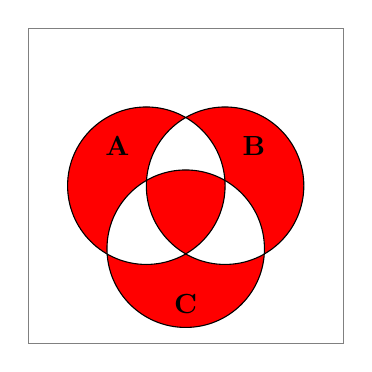
\begin{tikzpicture}
	\newcommand{\mycolor}{red}
	\newcommand{\mytextcolor}{blue}
	\newcommand{\myformulacolor}{gray}
	
		\def\universe{(-2.0,-2) rectangle (2.0,2)};
		\def\setA{(-0.5,0) circle (1)}
		\def\setB{(0.5,0) circle (1)}
		\def\setC{(0,-0.8) circle (1)}

		\draw[step=1.0cm,gray] \universe;
		
		\begin{scope}
			\fill[\mycolor] \setA;
			\fill[\mycolor] \setB;
			\fill[\mycolor] \setC;
			\begin{scope}[even odd rule]
			\clip \setB;
			\fill[white] \setA;
			\end{scope}
			\begin{scope}[even odd rule]
			\clip \setC;
			\fill[white] \setA;
			\end{scope}
			\begin{scope}[even odd rule]
			\clip \setB;
			\fill[white] \setC;
			\end{scope}
			\begin{scope}[even odd rule]
			\clip \setC \setB \setA;
			\fill[\mycolor] \setA;
			\end{scope}
		\end{scope}
		\draw \setA node[above left] {};
		\draw \setB node[above right] {};
		\draw \setC node[below] {};
		\node at (150:1)	{\textbf{A}};
		\node at (30:1)	{\textbf{B}};
		\node at (-90:1.5)	{\textbf{C}};
	\end{tikzpicture}
	
	% 5
	\solution \begin{align*}
		\overline{\overline{A}} &\IFF \{x\in U\st x\not\in \overline{A}\} && \text{(definition of complement)}\\
		&\IFF \{x\in U\st \NOT(x\in \overline{A})\} && \text{(definition of $\not\in$)}\\
		&\IFF \{x\in U\st \NOT(x\not\in A) \} && \text{(definition of complement)}\\
		&\IFF \{x\in U\st \NOT\NOT(x\in A)\} && \text{(definition of $\not\in$)}\\
		&\IFF \{x\in U\st x\in A\} && \text{(definition of double negation)}\\
		&\IFF A\\ \\
		A\cup \overline{A} &\IFF \{x \in U\st x\in A \OR x\in \overline{A}\} &&\text{(definition of $\cup$)}\\
		&\IFF \{x\in U\st x\in A \OR x\not\in A\} && \text{(definition of complement)}\\
		&\IFF \{x\in U\st x\in A \OR \NOT(x\in A)\} && \text{(definition of $\not\in$)}\\
		&\IFF \{x\in U\st \T\} &&\text{(excluded middle ($p\OR \NOT p\equiv \T$))}\\
		&\IFF U 
	\end{align*}
	
	% 6
	\solution\begin{align*}
	\overline{A\cap B} &\IFF \{x\in U\st x\not\in A\cap B \} &&\text{(definition of complement)}\\
	&\IFF \{x\in U\st \NOT (x\in A\cap B)\} &&\text{(definition of $\not\in$)}\\
	&\IFF \{x\in U\st \NOT (x\in A\AND x\in B)\} &&\text{(definition of $\cap$)}\\
	&\IFF \{x\in U\st (\NOT (x\in A))\OR (\NOT (x\in B))\} &&\text{(DeMorgan's Law for logic)}\\
	&\IFF \{x\in U\st (x\not\in A)\OR (x\not\in B)\} &&\text{(definition of $\not\in$)}\\
	&\IFF \{x\in U\st (x\in\overline{A})\OR (x\in\overline{B})\}&&\text{(definition of complement)}\\
	&\IFF \overline{A}\cup\overline{B}&&\text{(definition of $\cup$)}
	\end{align*}

	% 7
	\solution \spart \begin{align*}
	(p\AND q)\IFF p&\equiv((p\AND q)\IMP p) \AND (p\IMP (p\AND q)) && \text{(definition of $\IFF$)}\\
	&\equiv (\NOT(p\AND q) \OR p)\AND (\NOT p \OR (p\AND q)) && \text{(definition of $\IMP$)}\\
	&\equiv (\NOT p \OR \NOT q \OR p)\AND ((\NOT p \OR p) \AND (\NOT p \OR q)) && \text{(DeMorgan's law and Distributive law)}\\
	&\equiv \T \AND (\NOT p\OR q) &&\text{($p\OR\NOT p\equiv \T$)}\\
	&\equiv p\IMP q &&\text{(definition of $\IMP$)}\\ \\
	(p\OR q)\IFF q&\equiv ((p\OR q)\IMP q) \AND (q\IMP (p\OR q)) && \text{(definition of $\IFF$)}\\
	&\equiv (\NOT (p\OR q) \OR q) \AND (\NOT q \OR (p\OR q)) &&\text{(definition of $\IMP$)}\\
	&\equiv (\NOT p\OR q)\AND \T &&\text{(DeMorgan's law and Distributive law)}\\
	&\equiv p\IMP q
	\end{align*}
	\spart In order to show that these three statements are equivalent, we show that $A\SUB~B \IMP A\cap B= A$, $A\cap B= A\IMP A\cup B= B$, and $A\cup B = B\IMP A\SUB B$:\begin{itemize}
		\item $A\SUB~B \IMP A\cap B= A$:\\
		We show this by contradiction, and therefore assume that $A\SUB B$ and that $A\cap B\neq A$. Because of the latter, we know that there is an element in $A$ which is not in $B$. However, this contradicts our assumption that $A\SUB B$, hence we know that the original implication is true.
		\item $A\cap B= A\IMP A\cup B= B$:\\
		We show this by contradiction, and therefore we assume that $A\cap B= A$ and $A\cup B\neq B$. From the latter, we know that there now exists an element in $A$ which is not in $B$, lets say $x$. However, this means that $x$ should also be excluded from $A\cap B$, and hence $A\cap B\neq A$, contradicting our assumption. Therefore, the original implication is true.
		\item $A\cup B = B\IMP A\SUB B$:\\
		We show this by contradiction, and therefore assume that $A\cup B = B$ and that $\NOT(A\SUB B)$. Because of the latter, there exists at least one element, let say $x$, such that $x\in A$ and $x\not\in B$. This means that $C=A\SETDIFF B\neq\emptyset$. However, this means that $A\cup B = B\cup C$. This contradicts our other assumption that $A\cup B = B$, which states that $A\cup B$ only contains elements of $B$, whereas we have derived that this is not possible. Because of this contradiction, we conclude that $A\cup B = B\IMP A\SUB B$.
	\end{itemize}
	Because we have shown that all three implications hold, we have now shown that the three statements are logically equivalent.
	
	
	% 8
	\solution\begin{align*}
	\overline{A}&\IFF \{x\in U\st x\not\in A\} &&\text{(definition of $\overline{A}$)}\\
	&\IFF \{x\st x\in U \AND x\not\in A\}\\
	&\IFF U\SETDIFF A&&\text{(definition of $\SETDIFF$)}\\ \\
	C\SETDIFF (A\cup B)&\IFF \{x\st x\in C \AND x\not\in (A\cup B)\} &&\text{(definition of $\SETDIFF$)}\\
	&\IFF \{x\st x\in C\AND\NOT (x\in (A\cup B))\}&&\text{(definition of $\not\in$)}\\
	&\IFF \{x\st x\in C\AND\NOT (x\in A\OR x\in B)\}&&\text{(definition of $\cup$)}\\
	&\IFF \{x\st x\in C \AND (x\not\in A \AND x\not\in B)\}&&\text{(DeMorgan's law)}\\
	&\IFF \{x\st (x\in C\AND x\not\in A)\AND (x\in C\AND x\not\in B)\}&&\text{(Distributive law)}\\
	&\IFF \{x\st (x\in C\SETDIFF A)\AND (x\in C\SETDIFF B)\}&&\text{(definition of $\SETDIFF$)}\\
	&\IFF \{x\st x\in (C\SETDIFF A)\cap (C\SETDIFF B)\}&&\text{(definition of $\cap$)}\\
	&\IFF (C\SETDIFF A)\cap (C\SETDIFF B)\\ \\
	C\SETDIFF (A\cap B)&\IFF \{x\st x\in C \AND x\not\in (A\cap B)\} &&\text{(definition of $\SETDIFF$)}\\
	&\IFF \{x\st x\in C\AND\NOT (x\in (A\cap B))\}&&\text{(definition of $\not\in$)}\\
	&\IFF \{x\st x\in C\AND\NOT (x\in A\AND x\in B)\}&&\text{(definition of $\cap$)}\\
	&\IFF \{x\st x\in C \AND (x\not\in A \OR x\not\in B)\}&&\text{(DeMorgan's law)}\\
	&\IFF \{x\st (x\in C\AND x\not\in A)\OR (x\in C\AND x\not\in B)\}&&\text{(Distributive law)}\\
	&\IFF \{x\st (x\in C\SETDIFF A)\OR (x\in C\SETDIFF B)\}&&\text{(definition of $\SETDIFF$)}\\
	&\IFF \{x\st x\in (C\SETDIFF A)\cup (C\SETDIFF B)\}&&\text{(definition of $\cup$)}\\
	&\IFF (C\SETDIFF A)\cup (C\SETDIFF B)
	\end{align*}

	% 9
	\solution\begin{align*}
	A\cup (A\cap B)&\IFF (A\cup A)\cap (A\cup B)&&\text{(Distributive law)}\\
	&\IFF A\cap (A\cup B)&&\text{(Idempotent law)}\\
	&\IFF A &&\text{($A\subseteq A\cup B$ (see 2))}
	\end{align*}

	% 10
	\solution\spart\begin{align*}
	X\cup (Y\cup X)&\IFF (X\cup (X \cup Y)) &&\text{(Commutative law)}\\
	&\IFF (X\cup X)\cup Y &&\text{(Associative law)}\\
	&\IFF X\cup Y &&\text{(Idempotent law)}
	\end{align*}
	\spart\begin{align*}
	(X\cap Y)\cap\overline{X}&\IFF (Y\cap X)\cap\overline{X}&&\text{(Commutative law)}\\
	&\IFF Y\cap (X\cap\overline{X})&&\text{(Associative law)}\\
	&\IFF Y\cap \emptyset&&\text{(Miscellaneous law $A\cap \overline{A}=\emptyset$)}\\
	&\IFF \emptyset &&\text{(Miscellaneous law $A\cap\emptyset=\emptyset$)}
	\end{align*}
	\spart\begin{align*}
	(X\cup Y)\cap \overline{Y}&\IFF(X\cap \overline{Y})\cup (Y\cap\overline{Y})&&\text{(Distribution law)}\\
	&\IFF (X\cap\overline{Y})\cup\emptyset&&\text{(Miscellaneous law $A\cap\overline{A}=\emptyset$)}\\
	&\IFF X\cap\overline{Y}&&\text{(Miscellaneous law $A\cup\emptyset = A$)}
	\end{align*}
	\spart\begin{align*}
	(X\cup Y)\cup (X\cap Y)&\IFF(X\cup (X\cap Y)\cup (Y\cup (X\cap Y))&&\text{(Distributive law)}\\
	&\IFF((X\cap X)\cup (X\cap Y))\cup((Y\cap X)\cup (Y\cap Y))&&\text{(Distributive law)}\\
	&\IFF (X\cup (X\cap Y))\cup ((Y\cap X)\cup Y)&&\text{(Idempotent law)}\\
	&\IFF X\cup Y&&\text{($A\subseteq A\cup B$ (see 2))}
	\end{align*}

	% 11
	\solution\spart\begin{align*}
	\overline{A\cup B\cup C}&\IFF \overline{A}\cap\overline{B}\cap\overline{C}&&\text{(Theorem 4.5)}
	\end{align*}
	\spart\begin{align*}
	\overline{A\cup B\cap C}&\IFF\overline{A}\cap\overline{B\cap C}&&\text{(DeMorgan's law)}\\
	&\IFF\overline{A}\cap(\overline{B}\cup\overline{C})&&\text{(DeMorgan's law)}
	\end{align*}
	\spart\begin{align*}
	\overline{\overline{A\cup B}}&\IFF\overline{\overline{A}\cap\overline{B}}&&\text{(DeMorgan's law)}\\
	&\IFF A\cup B&&\text{(DeMorgan's law)}
	\end{align*}
	\spart\begin{align*}
	\overline{B\cap\overline{C}}&\IFF\overline{B}\cup C&&\text{(DeMorgan's law)}
	\end{align*}
	\spart\begin{align*}
	\overline{A\cap\overline{B\cap\overline{C}}}&\IFF\overline{A\cap(\overline{B}\cup C)}&&\text{(DeMorgan's law)}\\
	&\IFF\overline{A}\cup \overline{(\overline{B}\cup C)}&&\text{(DeMorgan's law)}\\
	&\IFF\overline{A}\cup (B\cap\overline{C})
	\end{align*}
	\spart\begin{align*}
	A\cap\overline{A\cup B}&\IFF A\cap\overline{A}\cap\overline{B}&&\text{(DeMorgan's law)}\\
	&\IFF \emptyset\cap\overline{B}&&\text{(Miscellaneous law $A\cap\overline{A}=\emptyset$)}\\
	&\IFF\emptyset&&\text{(Miscellaneous law $A\cap\emptyset = \emptyset$)}
	\end{align*}

	% 12
	\solution\begin{proof}
		We give a proof by induction.  In the base case, $n=2$, the
		statement is that $\overline{X_1\cap X_2}=\overline{X_1}\cup\overline{X_n}$.
		This is true since it is just an application of DeMorgan's law for two sets.

		For the inductive case, suppose that the statement is true for $n=k$. Hence, we assume the induction hypothesis: $\overline{X_1\cap X_2\cap \cdots \cap X_{k}}=\overline{X_1}\cup\overline{X_2}\cup\cdots\cup\overline{X_{k}}$,
		for $X_1$, $X_2$,
		\dots, $X_{k+1}$ being any $k+1$ sets. Then we have:
		\begin{align*}
		\overline{X_1\cap X_2\cap \cdots \cap X_{k+1}}
		&= \overline{(X_1\cap X_2\cap \cdots \cap X_k) \cap X_{k+1}}\\
		&= \overline{(X_1\cap X_2\cap \cdots \cap X_k)}\cup\overline{X_{k+1}}\\
		&= (\overline{X_1}\cup\overline{X_2}\cup\cdots\cup\overline{X_k})\cup\overline{X_{k+1}}&&\text{(IH)}\\
		&= \overline{X_1}\cup\overline{X_2}\cup\cdots\cup\overline{X_{k+1}}
		\end{align*}
		In this computation, the second step follows by DeMorgan's Law for
		two sets, while the third step follows from the induction hypothesis. Therefore by the principle of induction we have
		proven the theorem.
	\end{proof}

	% 13
	\solution\begin{itemize}
		\item For any natural number $n\geq 2$ and any sets $Q, P_1, P_2,\ldots, P_n$: $Q\cap (P_1\cup P_2\cup \ldots \cup P_n)=(Q\cap P_1)\cup (Q\cap P_2)\cup\ldots\cup (Q\cap P_n)$\begin{proof}
			We proof this by using induction. In the base case, $n=2$, the statement is that $Q\cap (P_1\cup P_2)=(Q\cap P_1)\cup (Q\cap P_2)$. This is true since this is just an application of the Distributive law for three sets.

			For the inductive case, suppose that the statement is true for $n=k$, where $k$ is an arbitrary integer bigger or equal to $2$. Hence, we assume the induction hypothesis: $Q\cap (P_1\cup P_2\cup \ldots \cup P_k)=(Q\cap P_1)\cup (Q\cap P_2)\cup\ldots\cup (Q\cap P_k)$, for $Q$, $P_1, P_2,\ldots P_{k+1}$ being any $k+2$ sets. Then we have:
			\begin{align*}
				Q\cap (P_1\cup P_2\cup \ldots \cup P_{k+1})&=(Q\cap (P_1\cup P_2\cup \ldots\cup P_k))\cup (Q\cap P_{k+1})\\
				&=((Q\cap P_1)\cup (Q\cap P_2)\cup\ldots\cup (Q\cap P_k))\cup (Q\cap P_{k+1})&&\text{(IH)}\\
				&=(Q\cap P_1)\cup (Q\cap P_2)\cup\ldots\cup (Q\cap P_{k+1})
			\end{align*}

			In this computation, the second step follows by Distributive law for three sets, while the third step follows from the induction hypothesis. Therefore by the principle of induction we have proven the theorem.
		\end{proof}
		\item For any natural number $n\geq 2$ and any sets $Q, P_1, P_2,\ldots, P_n$: $Q\cup (P_1\cap P_2\cap \ldots \cap P_n)=(Q\cup P_1)\cap (Q\cup P_2)\cap\ldots\cap (Q\cup P_n)$\begin{proof}
		We proof this by using induction. In the base case, $n=2$, the statement is that $Q\cup (P_1\cap P_2)=(Q\cup P_1)\cap (Q\cup P_2)$. This is true since this is just an application of the Distributive law for three sets.

		For the inductive case, suppose that the statement is true for $n=k$, where $k$ is an arbitrary integer bigger or equal to $2$. $Q\cup (P_1\cap P_2\cap \ldots \cap P_k)=(Q\cup P_1)\cap (Q\cup P_2)\cap\ldots\cap (Q\cup P_k)$, for $Q$, $P_1, P_2,\ldots P_{k+1}$ being any $k+2$ sets. Then we have:
		\begin{align*}
		Q\cup (P_1\cap P_2\cap \ldots \cap P_{k+1})&=(Q\cup (P_1\cap P_2\cap \ldots\cap P_k))\cap (Q\cup P_{k+1})\\
		&=((Q\cup P_1)\cap (Q\cup P_2)\cap\ldots\cap (Q\cup P_k))\cap (Q\cup P_{k+1})&&\text{(IH)}\\
		&=(Q\cup P_1)\cap (Q\cup P_2)\cap\ldots\cap (Q\cup P_{k+1})
		\end{align*}

		In this computation, the second step follows by Distributive law for three sets, while the third step follows from the induction hypothesis. Therefore by the principle of induction we have proven the theorem.
	\end{proof}
	\end{itemize}
\end{solutions}

\section*{Solutions 4.4}
\begin{solutions}
	% 1
	\solution\begin{align*}
	A\times B&=\{(1,a), (1,b), (1,c), (2,a), (2,b), (2,c), (3,a),(3,b),(3,c),(4,a),(4,b),(4,c)\}\\
	B\times A&=\{(a,1),(a,2),(a,3),(a,4),(b,1),(b,2),(b,3),(b,4),(c,1),(c,2),(c,3),(c,4)\}
	\end{align*}

	% 2
	\solution\begin{align*}
	g\circ f=\{(a,c), (b,c),(c,b),(d,d)\}
	\end{align*}

	% 3
	\solution\begin{align*}
	B^A=&\{\{(a,0), (b,0), (c,0)\},
	\{(a,0), (b,0), (c,1)\},
	\{(a,0), (b,1), (c,0)\},
	\{(a,0), (b,1), (c,1)\},\\
	&\{(a,1), (b,0), (c,0)\},
	\{(a,1), (b,0), (c,1)\},
	\{(a,1), (b,1), (c,0)\},
	\{(a,1), (b,1), (c,1)\}\}
	\end{align*}

	% 4
	\solution
		\spart $f$ is not onto, as there exists no element $x$ in $\Z$ such that $f(x)=2x=3$, because this means that $x=1.5$, which is not an integer. However, it is one-to-one. Take two arbitrary $a$ and $b$ such that $f(a)=f(b)$. Hence, $2a=2b$, which can only be true if $a=b$.
		\spart $g$ is onto; take an arbitrary $y$ in $\Z$. Then there exists an $x$ for which $g(x)=y$, namely $x=y-1$ ($g(x)=g(y-1)=y-1+1=y$), which is integer and thus in $ \Z$. Moreover, $g$ is one-to-one as well. Take two arbitrary $a$ and $b$ such that $g(a)=g(b)$. Hence $a+1=b+1$, which can only be true when $a=b$.
		\spart $h$ is not onto, as there exists no element $x$ in $\Z$ such that $h(x)=x^2+x+1=4$. This is because $x^2+x+1=4\IFF x=\frac{\pm\sqrt{13}-1}{2}$, which is not an integer. It is not one-to-one either, as solving $x^2+x+1=a$ gives two solutions for every $a$. Let us take $a=3$, then both $x=-2$ and $y=1$ give $h(x)=h(y)=3$, however, $x\neq y$.
		\spart $s$ is onto; take an arbitrary $y\in\Z$. Then there exists an $x$ for which $s(x)=y$, namely $x=2y$ ($s(x)=s(2y)=\frac{2y}{2}=y$). However, it is not one-to-one. Take an arbitrary even integer $a$ and $b=a-1$. $s(a)=\frac{a}{2}=\frac{(a-1)+1}{2}=s(b)$, however, $a\neq b$.

	% 5
	\solution For any $x\in A$:
	\begin{align*}
	((h\circ g)\circ f)(x)=(h\circ g)(f(x))=(h(g(f(x))))=h((g\circ f)(x))=(h\circ (g\circ f))(x)
	\end{align*}

	% 6
	\solution\spart\textbf{To prove:} $g\circ f$ is one-to-one $\IMP f$ is one-to-one
	\begin{proof}
		We use proof by contradiction. We assume that $g\circ f$ is one-to-one, but $f$ is not. Because $f$ is not one-to-one, so there exists an $a,b\in A$ such that $f(a)=y=f(b)$, but $a\neq b$. However, since $g: B\to C$, we have an element $x\in C$ such that $g(y)=x$. However, this would mean that for both $a$ and $b$, $(g\circ f)(a)=(g\circ f)(b)=x$, showing that $g\circ f$ is not one-to-one. However, this contradicts our assumption that $g\circ f$ is one-to-one, which mean that it cannot hold that $g\circ f$ is one-to-one, but $f$ is not. Hence, the statement that has to be proven is true.
	\end{proof}
	\spart Let $A=\{1\}, B=\{a, b\}, C=\{c\}, f(1)=a, g(a)=g(b)=c$. Although $g$ is not one-to-one, as both $g(a)=g(b)=c$, we have that $g\circ f(1)=c$, which is one-to-one.

	% 7
	\solution\spart \textbf{To prove:} $g\circ f$ is onto $\IMP g$ is onto\begin{proof}
		We use proof by contradiction. We assume that $g\circ f$ is onto, but $g$ is not. Because $g$ is not onto, this means that there is an element $c\in C$ such that for all elements in $b\in B: g(b)\neq c$. However, this would mean that $g\circ f$ cannot be onto, as there is no element in $B$ that $f$ can map to such that $g\circ f(x)=c$. However, this contradicts our assumption that $g\circ f$ is onto, which mean that it cannot hold that $g\circ f$ is onto, but $g$ is not. Hence, the statement that has to be proven is true.
	\end{proof}
	\spart Let $A=\{a\}, B=\{b,c\}, C=\{d\}, f(a)=b, g(b)=d$. Although $f$ is not onto, as there is no $x\in A$ such that $f(x)=c$, we have that for all elements in $C$, namely $d$, that there exists an element in $A$, namely $a$, such that $(g\circ f)(a)=d$. Hence $g\circ f$ is onto.
\end{solutions}
